\documentclass[11pt]{beamer}
\usetheme{Pittsburgh}
\usepackage[utf8]{inputenc}
\usepackage{amsmath}
\usepackage{amsfonts}
\usepackage{pifont}
\newcommand{\cmark}{\ding{51}}%
\newcommand{\xmark}{\ding{55}}%
\usepackage{amssymb}
\usepackage{todonotes}
\usepackage{ragged2e} 
\usepackage{comment}
\usepackage{enumitem}
\usepackage{tikz}
\usepackage{pgfgantt} 
\usepackage{listings}
\setcounter{tocdepth}{2}% Allow only section(1) and subsection(2), no subsubsection (3), in ToC

\setlist[itemize]{label=\textcolor{blue}{\textbullet}}
\newcommand{\xitem}{\item[\textcolor{red}{\xmark}]}
\newcommand{\citem}{\item[\textcolor{olive}{\cmark}]}

\author{Benjamin Rüth}
\title{Bokeh: A Python Plotting Library for the Web Browser}
\subtitle{Presentation at Chair of Structural Mechanics, BGU, TUM}
%\setbeamercovered{transparent} 
\setbeamertemplate{navigation symbols}{}%remove navigation symbols
%\logo{} 
%\institute{} 
\date{\today} 
%\subject{} 

\newcommand{\mytexttt}[1]{\colorbox{gray!20}{\texttt{#1}}}

\AtBeginSection[]
{
  \begin{frame}
    \frametitle{Table of Contents}
    \tableofcontents[currentsection]
  \end{frame}
}

\begin{document}
\setbeamertemplate{caption}{\raggedright\insertcaption\par}

\begin{frame}
\titlepage
\end{frame}

\section{Why do we need web visualization?}
\begin{frame}
\frametitle{\insertsection}
\textbf{Phase Plane Pictures: Source, Sink, Saddle}\\
Gilbert Strang, MIT\footnote{\url{https://www.youtube.com/watch?v=VqXKa11IA6A}}
\begin{center}
\only<1>{
the task\\
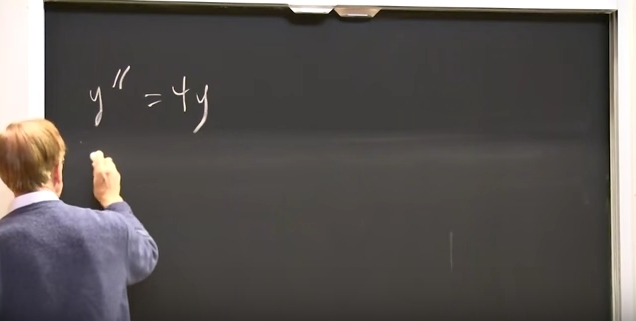
\includegraphics[width=.8\textwidth]{Pictures/Strang1.jpg}}
\only<2>{
3 minutes later\\
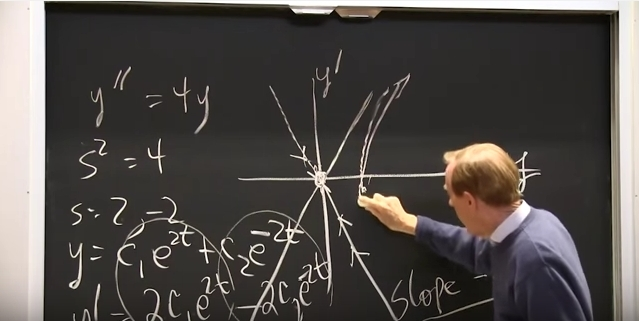
\includegraphics[width=.8\textwidth]{Pictures/Strang2.jpg}}
\only<3>{
another 2 minutes later\\
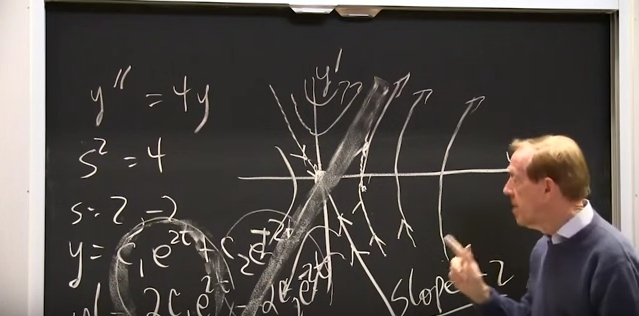
\includegraphics[width=.8\textwidth]{Pictures/Strang3.jpg}}
\end{center}
\end{frame}

\begin{frame}
\frametitle{\insertsection}
\begin{center}
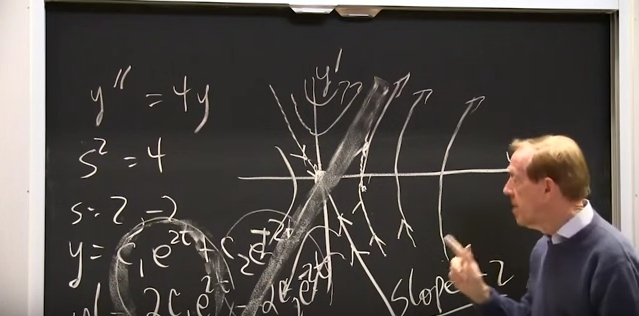
\includegraphics[width=.8\textwidth]{Pictures/Strang3.jpg}
\end{center}
\begin{block}{Problem with Videos and Lectures}
\begin{itemize}
\item Advisor needed
\item Time intensive
\item Not interactive (videos)
\item Not individual
\end{itemize}
\end{block}
\end{frame}

\section{Interactive Web Visualization}

\subsection{What do we want?}
\begin{frame}
\frametitle{\insertsubsection}
\begin{block}{Our goal}
\begin{itemize}
\item Visualization of math \& mechanics content
\item Easy-to-use, flexible tool
\item For use at home and in lectures
\end{itemize}
\end{block}
\pause
\begin{block}{User Constraints}
\begin{itemize}
\item No programming experience required
\item No special tools required
\end{itemize}
\end{block}
\pause
\begin{block}{Development Constraints}
\begin{itemize}
\item Easy to implement and understand
\item Support for scientific applications
\end{itemize}
\end{block}

\end{frame}

\subsection{Setup and Tools}
\begin{frame}
\frametitle{\insertsubsection}
\begin{block}{Installation}
\begin{itemize}
\item \textbf{Version Control:} Git \\
{\footnotesize\url{https://git-scm.com/downloads}}
\item \textbf{Python:} Anaconda \\
{\footnotesize\url{https://www.continuum.io/downloads}}
\item \textbf{IDE:} install PyCharm \\
{\footnotesize\url{https://www.jetbrains.com/pycharm/}}
\end{itemize}
\end{block}
\end{frame}

\begin{frame}
\frametitle{\insertsubsection}
\begin{block}{Git: Working on software in a team}
\begin{itemize}
\item \mytexttt{git clone} for downloading the source
\item \mytexttt{git pull/push} for syncing with the repository
\item \mytexttt{git add/commit} for contributing
\item \mytexttt{git branch} for experiments
\end{itemize}
\end{block}

\pause

\begin{block}{Our repository:}
\begin{itemize}
\item Sign up on \url{https://github.com/}
\item \url{https://github.com/BenjaminRueth/Visualization}
\item \textbf{HTTPS:} \\
{\footnotesize\mytexttt{git clone https://github.com/BenjaminRueth/Visualization.git}}
\item \textbf{SSH:\footnote{here you need a SSH key! \\ {\scriptsize\url{https://help.github.com/articles/connecting-to-github-with-ssh/}}}} \\
{\footnotesize\mytexttt{git clone git@github.com:BenjaminRueth/Visualization.git}}
\end{itemize}
\end{block}
\end{frame}

\begin{frame}
\frametitle{\insertsubsection}
\begin{block}{Anaconda: A Python distribution}
\begin{itemize}
\item \textbf{Anaconda prompt:} \mytexttt{conda install bokeh}
\item \textbf{Python prompt:} \mytexttt{ipython} or \mytexttt{python}
\end{itemize}
\end{block}
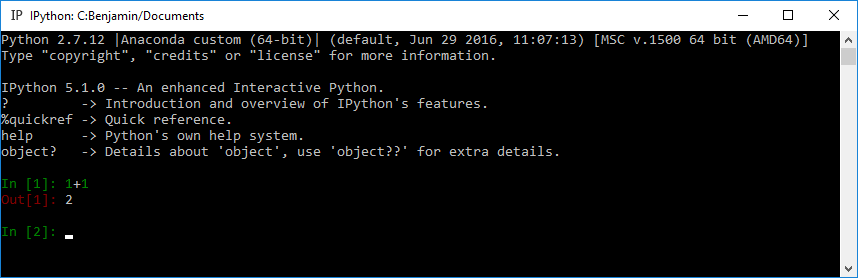
\includegraphics[width = \textwidth]{Pictures/PythonShell.png}
\end{frame}

\section{Bokeh}
\subsection{Introduction to Bokeh}
\begin{frame}
\frametitle{\insertsubsection}
\begin{figure}
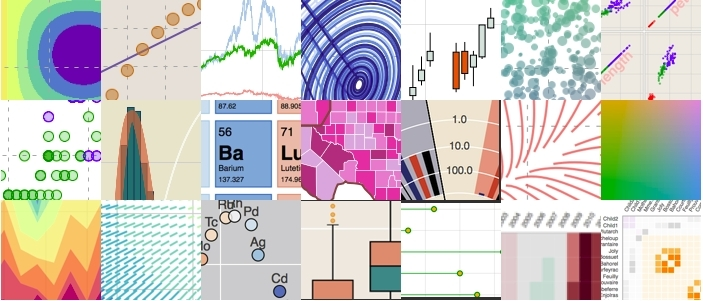
\includegraphics[width=.8\textwidth]{Pictures/bokehGallery.jpg}
\end{figure}
\begin{itemize}
\item Python plotting library (similar to matplotlib)
\item uses the webbrowser for displaying graphics
\item uses \texttt{D3.js}
\item open source
\item visit \url{http://bokeh.pydata.org}
\end{itemize}
\end{frame}

\begin{frame}
\frametitle{\insertsubsection}
\begin{block}{Necessary preparations}
\begin{itemize}
\item \textbf{Clone the repository:} \\
use Git.
\item \textbf{Our working directory:} \\
\mytexttt{...\textbackslash Visualization\textbackslash Presentation\textbackslash Examples}
\item \textbf{Start a shell:} 
\begin{itemize}
\item \textbf{Windows:} \mytexttt{start+r}, then type \text{cmd}
\item \textbf{Linux:} \mytexttt{ctrl+alt+T}
\item with \mytexttt{cd <path>} navigate to the working directory
\end{itemize}
\end{itemize}
\end{block}
\end{frame}

\begin{frame}[fragile]
\frametitle{\insertsubsection}
\begin{block}{Static example: Plotting in the browser}
\begin{itemize}
\item Fire up a shell in your working directory
\item Start with \mytexttt{python staticPlotting.py}
\item The browser should show the plot
\end{itemize}
\end{block}
\end{frame}

\begin{frame}[fragile]
\frametitle{\insertsubsection}
\begin{block}{Static example: Plotting in the browser}
\lstinputlisting[
commentstyle=\textbf,
language=Python,
basicstyle=\footnotesize]
{Examples/staticPlotting.py}
\end{block}
\end{frame}

\begin{frame}
\frametitle{\insertsubsection}
\begin{block}{Server example: An interactive function plotting tool}
\begin{itemize}
\item Fire up a shell in your working directory
\item Start with \mytexttt{bokeh serve functionPlotter.py}
\item Visit \url{http://localhost:5006/functionPlotter}
\pause
\item only 60 LoC!
\item uses \texttt{numpy} and \texttt{scipy}
\end{itemize}
\end{block}
\end{frame}

\begin{frame}
\lstinputlisting[
commentstyle=\textbf,
language=Python,
basicstyle=\footnotesize]
{Examples/functionPlotterShort.py}
\end{frame}

\subsection{Example: Phase Plane Pictures}
\begin{frame}
\frametitle{\insertsubsection}
\begin{figure}
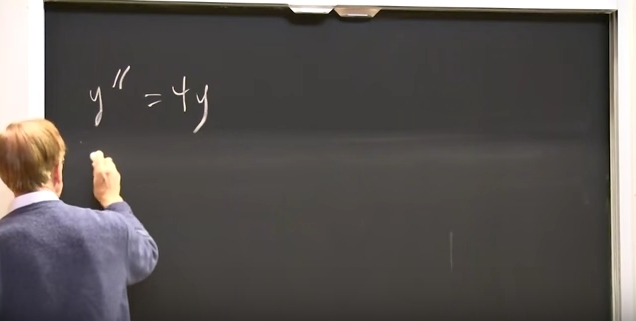
\includegraphics[width=.7\textwidth]{Pictures/Strang1.jpg}
\end{figure}
\pause
\begin{block}{2D ODE system}
\begin{align*}
y'' = u(x,y) & = 4y \\
y' = v(x,y) & = x
\end{align*}
Visualization on \url{http://localhost:5006/odesystem_app}
\end{block}
\end{frame}

\subsection{What do we get?}
\begin{frame}
\frametitle{\insertsubsection}
\begin{center}
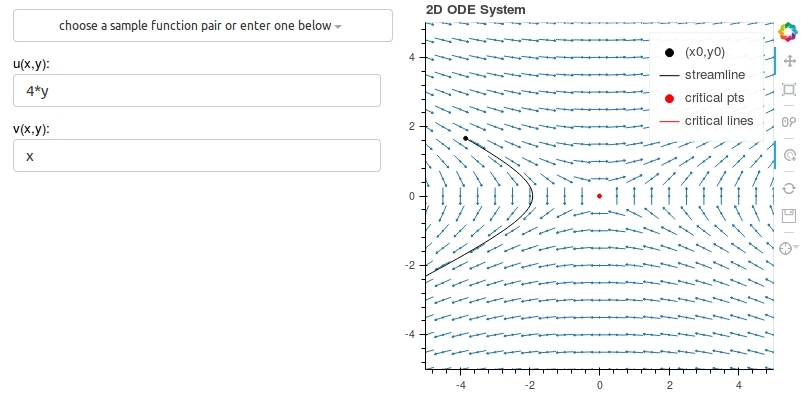
\includegraphics[height=.5\textheight]{Pictures/PhasePortraitPlot.jpg}
\end{center}
\begin{block}{Our goal}
\begin{itemize}
\citem Visualization of math (\& mechanics?) content
\citem Easy-to-use, flexible tool
\citem For use at home and in lectures
\end{itemize}
\end{block}

\end{frame}

\begin{frame}
\frametitle{\insertsubsection}
\begin{block}{User Constraints}
\begin{itemize}
\citem No programming experience required
\citem No special tools required
\end{itemize}
\end{block}

\begin{block}{Development Constraints}
\begin{itemize}
\citem Easy to implement and understand
\citem Support for scientific applications
\end{itemize}
\end{block}

\begin{block}{BUT}
\begin{itemize}
\item we need a server
\item the user needs an internet connection
\item we have to transfer data
\item sometimes slow
\end{itemize}
\end{block}
\end{frame}

\section{Collaborating}
\frametitle{\insertsubsection}
\begin{frame}
\begin{block}{Use Git}
\begin{itemize}
\item \textbf{Create a branch:} \mytexttt{git checkout -b <myName>}
\item \textbf{Develop:} e.g. change something in \mytexttt{Visualization/Example/staticPlotting.py}
\item \textbf{Finalize:} \mytexttt{git add}, \mytexttt{git commit -m "..."}
\item \textbf{Synchronize:} \mytexttt{git push}\footnote{probably you get the hint to type:\\
\mytexttt{git push --set-upstream origin <myName>} just do it.}
\item \textbf{Merge:} \mytexttt{git checkout master}, \mytexttt{git merge <myName>}
\end{itemize}
\end{block}
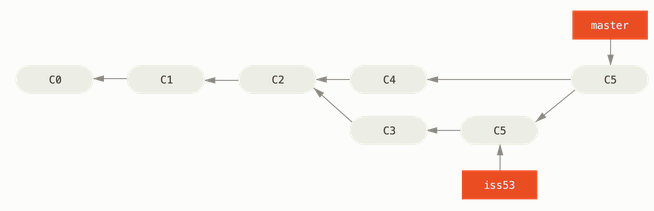
\includegraphics[width=\textwidth]{Pictures/branching.png}
\end{frame}

\begin{frame}
\begin{columns}
\begin{column}{.5\textwidth}
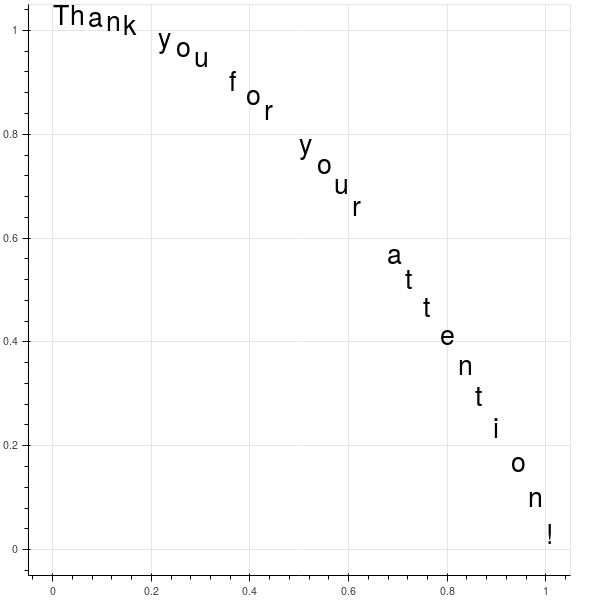
\includegraphics[width=\textwidth]{Pictures/thanks.png}
\end{column}
\begin{column}{.5\textwidth}
\lstinputlisting[
commentstyle=\textbf,
language=Python,
basicstyle=\tiny]{Examples/thanks.py}
\end{column}
\end{columns}

\end{frame}

\end{document}
